\titleformat{\section}{\normalfont\Large\bfseries}{\chaptertitlename\ \thechapter:}{0.5em}{}

\addcontentsline{toc}{chapter}{Appendix}
% \chapter*{Appendix}
\clearpage

\newcommand{\appendixsection}[1] {
    \addtocounter{chapter}{1}
    \section{#1}
}

\appendixsection{Chemical composition of AFFF}
\begin{table}[H]
    \centering
    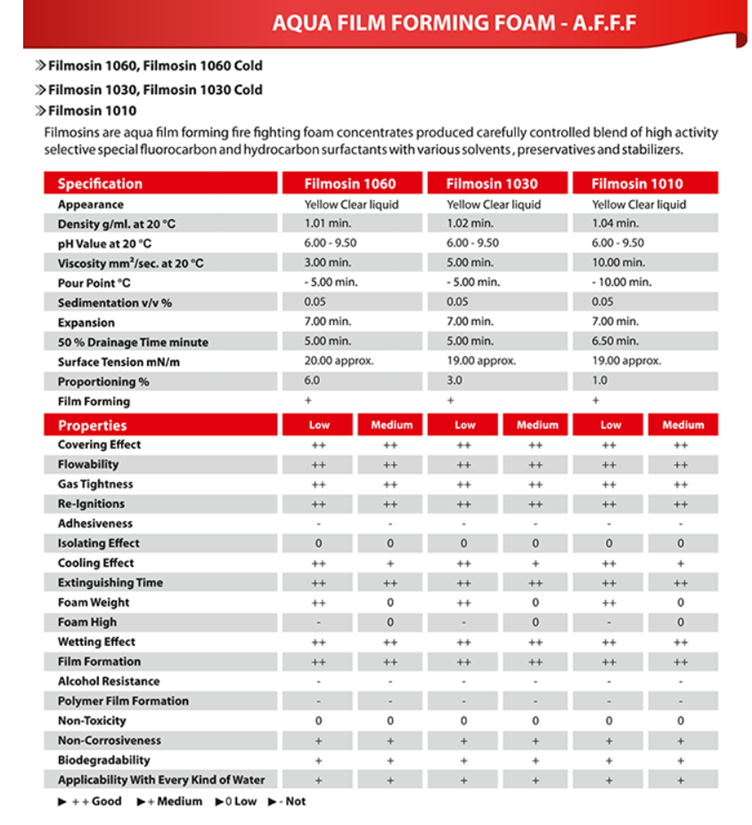
\includegraphics[width=\textwidth]{original_composition_of_afff_concentrate.png}
    \caption{Original composition of AFFF concentrate \cite{hinnant2020characterizing}.}
\end{table}

\appendixsection{Properties and composition of steels}
\begin{table}[H]
    \centering
    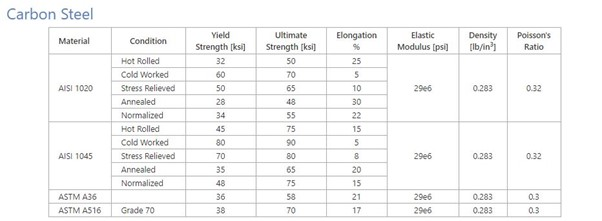
\includegraphics[width=\textwidth]{mechanical_and_physical_properties_of_mild_steel.jpg}
    \caption{Mechanical and physical properties of mild steel (AISI 1020) \cite{kabir2020critical}}
\end{table}

\begin{table}[H]
    \centering
    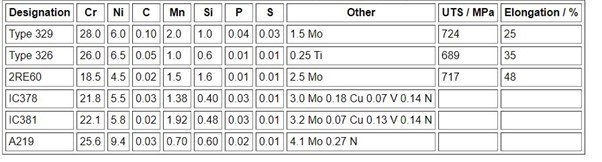
\includegraphics[width=\textwidth]{weighed_composition_of_duplex_stainless_steel.jpg}
    \caption{Weighed composition of duplex stainless steel \cite{sourmail2005stainless}}
\end{table}

\begin{table}[H]
    \centering
    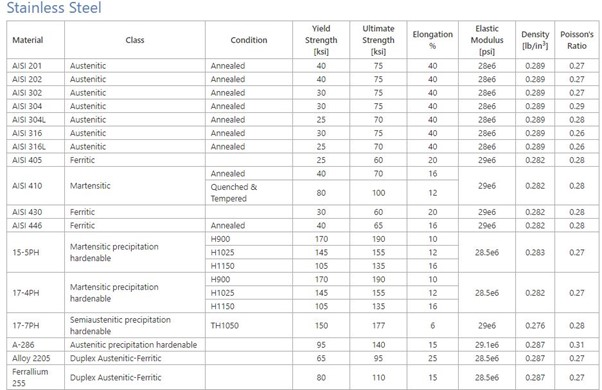
\includegraphics[width=\textwidth]{mechanical_and_physical_properties_of_stainless_steel.jpg}
    \caption{Mechanical and physical properties of stainless steel \cite{bhadeshia2017steels}}
\end{table}

\appendixsection{Role of microstructural constituents}
\begin{table}[H]

\fontsize{10}{12}\selectfont
\renewcommand{\arraystretch}{1.2}

\centering
\begin{tabular}{p{.2\textwidth} m{.4\textwidth} m{.4\textwidth}}
\hline
Microstructural constituents & Dependent on/characteristics(selection) & Responsible for (examples) \\
\hline
Vacancies & Temperature, deformation & Hardening at low temperatures; diffusion processes at elevated temperatures; diffusional creep \\
Dislocations & Deformation, temperature, recovery and recrystallization processes; at elevated temperatures edge dislocations may climb, and leave their slip planes & Plastic deformation strength is controlled by their number and motion; driving force for recrystallization; dislocation creep \\
Stacking faults & Crystal structure, alloying & Mobility of dislocations, for example, climb of edge dislocations and cross-slip of screw dislocations is hampered \\
Mechanical twins & Stacking fault energy, deformation, temperature & Additional deformation mechanism at low temperatures and/or high strain rates \\
Subgrains/domains & Deformation, temperature, stacking fault energy/ordered crystal structure; antiphase boundary energy & Work hardening, creep, creation of antiphase boundaries \\
Grain boundaries & Lattice orientation between neighboring grains; subdivision in small-angle, medium-angle and high-angle grain boundaries & Work hardening by acting as barries to slip from one grain to the next; segregation site of impurity atoms \\
Phase boundaries & Alloy system, composition, phase stability at elavated temperatures & Strengthening effects, for example, in duplex or multiphase steels\\
Grains & Alloy system, type of nucleation, processing, deformation, heat treatment, recrytallization & Strengthening (see grain boundaries) but ductility is maintained; grain boundary sliding at elavated temperatures (creep, superplasticity)\\
Annealing twins & Stacking fault energy; characteristic of face-cenntered cubic materials exhibiting a low stacking fault energy & Lowering of total boundary energy during grain growth \\
Precipitates / dispersoids & Alloy system, composition, heat treatment, processing; the interface between particle and matrix can be coherent, semicoherent, or incoherent & Increase in strength by the interaction of moving dislocation; dislocations can loop, cut through or cross-slip the particles at ambient temperatures; at elevated temperatures the dislocations can surmount the particles by climb processes\\
\end{tabular}

\caption{Role of microstructural constituents on metallic materials \cite{suryanarayana2017microstructure}.}
\label{appendix:c:5}
\end{table}

\appendixsection{Full annealing temperature cycle}
\begin{table}[H]
    \centering
    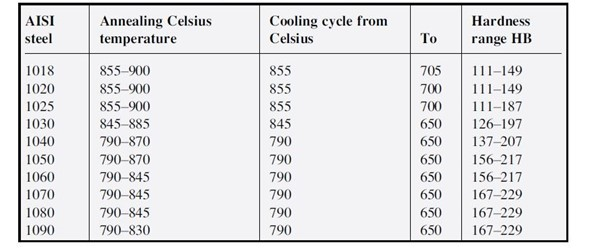
\includegraphics[width=\textwidth]{full_annealing_temperature_cycle.jpg}
    \caption{Full annealing temperature cycle of popular steel and hardness range \cite{singh2020applied}}
\end{table}

\appendixsection{Effect of changing various substances in PE}
\begin{table}[H]
    \centering
    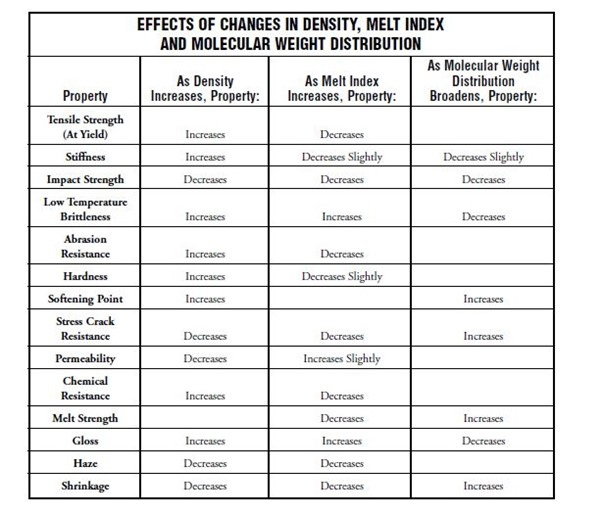
\includegraphics[width=\textwidth]{effect_of_changes_on_properties_of_pe.jpg}
    \caption{The effect of changes in density, melt index, and molecular weight distribution on the properties of PE \cite{gabriel1998history}}
\end{table}

\begin{table}[H]
    \centering
    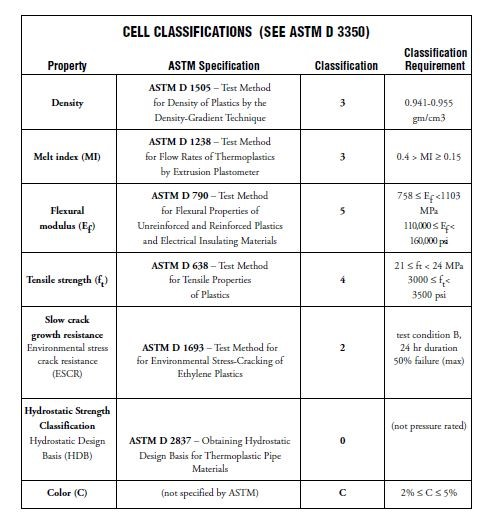
\includegraphics[width=\textwidth]{cell_classifications_for_pe.jpg}
    \caption{Cell classifications for PE \cite{meola2005cross}.}
\end{table}